Im Versuch wird der Ultraschall mit einem Ultraschallechoskop erzeugt und auf einem Rechner visualisiert. Das Computerprogramm zeigt die detektierte Spannung in Abhängigkeit von der Zeit. Wird die Schallgeschwindigkeit des Mediums dort eingetragen, kann auch die Tiefe des betrachteten Körpers angezeigt werden. Als Kontaktmittel zwischen verschiedenen Körpern bzw. den Körpern und den Ultraschallsonden wird Wasser oder Ultraschallgel verwendet. \\
Im ersten Versuchsteil werden \textbf{Zylinder aus Acrylglas} verwendet. Zunächst werden ihre Höhen mit einer Schieblehre ermittelt. Danach wird für einen Zylinder die Reflexionsamplitude ermittelt. Schließlich wird die Durchlaufzeit einiger Zylinder(-kombinationen) sowohl mit der Impuls-Echo- als auch mit der Durchschallungsmethode gemessen. \\
Im zweiten Teil sollen Mehrfachechos detektiert werden. Dafür wird ein Zylinder auf zwei unterschiedlich dicke \textbf{Acryl-Glas-Quader} gestellt. Hierbei treten an jeder Grenzfläche Reflexionen auf, sodass Wellen an der Sonde ankommen, die mehrfach reflektiert wurden. In der Anzeige im Computerprogramm sollen die Mehrfachreflexionen in den Quadern angezeigt werden. Durch den Zylinder werden die Peaks der Mehrfachreflexionen in der Zeit verschoben, sodass sie besser unterscheidbar sind. Mit Hilfe des Computerprogramms wird diese Anzeige zwei Mal fouriertransformiert, um ein glatteres Bild zu erhalten.\todo[color=red]{Das habe ich immer noch nicht verstanden.} \\
Zuletzt wird das \textbf{Modell eines menschlichen Auges} mit der Impuls-Echo-Methode vermessen. Dabei ist darauf zu achten, dass die Bauteile verschiedene Schallgeschwindigkeiten haben.
\begin{figure}[h!]
	\centering
	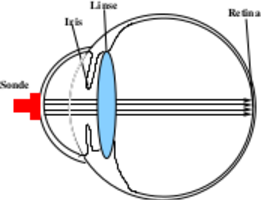
\includegraphics[width=0.4\textwidth]{Auge.pdf}
	\caption{Verwendetes Modell des Auges}
	\label{fig:Auge}
\end{figure}\todo[color=red]{Problembild}